\documentclass{article}
	\usepackage[UKenglish]{babel}
	\usepackage{url}
	\usepackage[T1]{fontenc}
	\usepackage{lineno} % used in genre
	\usepackage{booktabs}
	\usepackage{graphicx}
	\usepackage{setspace}
	\usepackage{tabularx}
	\usepackage{multicol}
	\usepackage{comment}
	\usepackage{graphics}
	\usepackage[hidelinks]{hyperref}
	\usepackage[backend=biber,style=apa,apamaxprtauth=7,doi=false,isbn=false,uniquename=false,url=false,bibencoding=utf8]{biblatex}
	\DeclareLanguageMapping{british}{british-apa}
	% no notes ??
	\AtEveryBibitem{%
	  \clearfield{note}%
	}
	\usepackage{xparse}
	\usepackage{csquotes}
	\usepackage[open]{bookmark}
	\addbibresource{references.bib}
	\newcommand{\citeNP}{\cite}
	\renewcommand{\cite}{\parencite}
	% make sure there's a comma after and in refs like proper apa
	\AtBeginDocument{\renewcommand\finalandcomma{\addcomma}}
	\AtBeginBibliography{%
	  \renewcommand*{\finalnamedelim}{%
	    \ifthenelse{\value{listcount}>\maxprtauth}
	      {}
	      {\finalandcomma\addspace\&\space}}}
	\author{Daniel McDonald}
	\date{\today}
	\title{Diagnosis discourses in an online bipolar community: a mixed-methods approach}
	\begin{document}
	\maketitle

%%%%%%%%%%%%%%%%%%%%%%%%%%%%%%%%%%%%%%%%%%%%%%%%%%%%%%
%%%%%%%%%%%%%%%%% ARTICLE CONTENT %%%%%%%%%%%%%%%%%%%%
%%%%%%%%%%%%%%%%%%%%%%%%%%%%%%%%%%%%%%%%%%%%%%%%%%%%%%

\begin{abstract}
	Online support groups provide a popular means of exchanging health information and social support with others. Often, new members to these communities provide a self-introduction, giving a narrative account of their healthcare journey. Common in both these newcomer narratives and in other members' responses is discussion of \emph{diagnosis} by a healthcare professional, or lack thereof. This paper describes an investigation of talk about diagnosis in new and veteran members' contributions to a large online bipolar disorder community, incorporating a systemic-functional conceptualisation of genre and transitivity. The analysis is a mixed-methods one: qualitative analysis of posts within a newcomers' thread highlights how diagnosis is construed and negotiated within a single text. This is then complemented by a corpus linguistic analysis, which charts changes in the syntagmatic behaviour of \emph{diagnose} as a verb, as well as trends toward nominalisation. The affordances of computational methods in health discourse analysis are highlighted. Future directions, opened up by the largely automated research design, are then briefly discussed.
	\end{abstract}

\section{Context: online health communities}

	It is well-established that the Internet is a popular source and vast repository of health information. Of particular interest to linguistic research in the past two decades has been interactional sites of health information exchange such as online support groups (OSGs): websites (or parts thereof) where users can post and reply to text-based threads. Forum-based OSGs vary widely in terms of their medium (i.e. technological) and situation (i.e. socially prescribed) affordances \cite{herring_faceted_2007}: In many cases, they can be viewed without logging in, and their threads are returned in search engine queries. Posting and replying to threads, however, usually involves creating an account. Some have strict moderation and can enforce bans; some allow users to embed images and videos into posts; some allow users to create profiles and send private messages \cite{morzy_analysis_2012}. Having remained in use since their beginnings in the 1990s, these forums have a long research history \cite[e.g.][]{sharf_communicating_1997}. That said, there is also growing evidence that the popularity of online forums is in decline, with consumers instead receiving information and support from social networking sites (e.g. \emph{Facebook}), link\slash content aggregation platforms (e.g. \emph{Reddit}) or any of countless dedicated mobile apps (for diet and weight management, exercise, smoking cessation, and so on).

	When compared with face-to-face support groups, OSGs may have unique benefits and consequences for users' health. In terms of benefits, forum users generally have round-the-clock access to a global community, facilitating larger groups and constant support \cite{stommel_online_2010,stommel_use_2011}. This support has been linked to improved understanding of illness, the development of coping strategies, reduced anxiety and depression, and an increasing confidence in health professionals \cite{mulveen_interpretative_2006,swan_sharing_2010,manchaiah_use_2013,yao_impact_2015}. Furthermore, the degree of anonymity in such environments has sometimes been found to lead to a disinhibiting effect, encouraging honest discussion \cite{mo_are_2013} with qualitative differences from professional--consumer and\slash or face-to-face interactions \cite{maclean_forum77:_2015}. Of concern to some researchers, however, has been the potential spread of misinformation due to non-expert advice \cite{ziebland_how_2004}. Regular forum members may gain expert status within OSGs despite a lack of formal medical credentials \cite{hardey_doctor_1999,thompson_credibility_2012}. Such concerns are compounded in situations involving vulnerable participants who may not have the ability to make sound decisions regarding their own health.
	% not sure if needed:
	Finally, forum cultures may have the effect of normalising mental health issues such as suicidal ideation and eating disorders, and may encourage users to exhibit symptoms or obtain diagnoses for the purposes of legitimating themselves socially within the community \cite{horne_doing_2009,vayreda_social_2009}. These issues have been hypothesised to be the result of the dual function of OSGs as sites for both health information and social support exchange \cite{nambisan_information_2011,attard_thematic_2012}.

	For researchers, OSGs provide a unique window into the consumer healthcare journey \cite{harvey_disclosures_2012}. First, as noted above, situation factors present in OSGs (i.e. the informal, intra-consumer tenor of interactions) lead to texts that construe the consumer journey candidly, in detail, and unadulterated by potential influence of healthcare professionals. At the same time, the medium factors of OSGs (i.e. the way the interactions are produced and archived) make viable the use of state-of-the-art computational linguistic methods: because OSGs are generally anonymous, large, well-structured and metadata-rich, they can be automatically transformed into high-quality corpus linguistic resources, grammatically annotated, and searched using tools and methods from corpus linguisics (CL).


\subsection{Language use in online support groups} \label{sect:intro-lang-in-osg}

	In OSGs, language is the dominant resource through which meanings are made. Accordingly, OSG research almost always involves some level of analysis of the language use of forum members, with or without explicit reference to linguistic theory. Legitimation research, for example, has focussed on the ways in which newcomers construct an identity and message that warrants useful responses from others \cite{galegher_legitimacy_1998,west_facework_2010}. Depending on the community, legitimation strategies have been found to vary widely: newcomers may emphasise the severity and uniqueness of their case , stress their inexperience and need for guidance, or present evidence that they fit normative biomedical understanding of the pathology (i.e. exhibiting symptoms) or the healthcare journey (having been diagnosed) \cite{varga2014grieving,smithson_membership_2011}. Another common approach to understanding online communities is socialisation---that is, how users learn through participation in meaningful social interaction with more experienced members of groups \cite{ochs_socialization_1991}. \textcite{lee_new_2014}, for example, approach socialisation from a member-life-cycle perspective, arguing that members transition through a number of roles during their time within the online community, and that each role has accompanying needs and responsibilities. Newcomers have strong needs for both information and social support, but may not contribute due to the potential for loss-of-face if information they provide is judged by experts to be incorrect \cite{fuller_innovation_2007} or at odds with community-specific values \cite{weber_missed_2011}. At later stages in the member life-cycle, users become less anxious about producing content, but lose the motivation to seek out information or support \cite{lee_new_2014}. Within this literature, lacking so far have been accounts of the longitudinal evolution of role-relationship negotiation strategies, comparisons of new and veteran users' linguistic choices, quantitative approaches, and attempts to map longitudinal change in discourse and semantics to shifts in lexicogrammatical features.

	Another useful area investigating language use and health is \emph{consumer-centred medicine} research \cite{stewart_effective_1995}. Under this paradigm, clinicians foster collaborative exchanges with those they treat: greater attention is paid to consumers' feelings and beliefs; consumers are actively involved in decision-making processes; clinicians establish long-term relationships that can be responsive to consumers' prior journeys through the healthcare system \cite{woodward-kron_international_2016}. The consumer-centred model thus recognises the centrality of communication and interaction to the practice of medicine, necessitating functional linguistic analysis of healthcare communication%---that is, research into the relationship between language use in healthcare and more effective healthcare practice.
	So far, however, healthcare communication research has typically focussed on clinician--consumer interactions within formal settings, such as hospitals and clinics \cite{slade_communicating_2015}. Despite acknowledgement that the consumer journey extends far beyond his\slash her interactions with healthcare professionals \cite{balka_situating_2010,dickerson_cancer_2011}, and despite the increasing prominence of the interactional Web in daily life \cite{hadlington_cognitive_2015}, little has been done to connect consumers' interactions with clinicians to their use of OSGs.

\subsection{New members' contributions to OSGs}

A great deal of OSG research has focussed on analysis of newcomers' interactions. Because drop-out rates in online communities are generally high, such `first post threads' are a constant feature in the landscape of many popular forums. A synthesis of literature shows that there are broad interpersonal similarities between first contributions within many OSGs. Generally speaking, new users attempt to carve out a social position from which it is possible to elicit certain kinds of language from others---that is, to increase the perlocutionary force of one's own utterances \cite{austin_how_1975,roberts_communicative_1996}. Most commonly, new users want to be given information and social support after having requested it. This has been referred to as a position of legitimacy, arrived at through an ongoing process of \emph{legitimation} through semiotic exchange \cite{davies_communities_2005,smithson_developing_2012,van_leeuwen_legitimation_2007}. In comparison to offline support groups, where physical co-presence and extralinguistic communication can serve legitimating functions, new contributors to OSGs instead exchange meaning and communicate legitimacy almost exclusively through the linguistic content of their posts \cite{galegher_legitimacy_1998}. The kinds of language choices that manoeuvre the user into the legitimate position may vary, with individual community cultures shaping what messages contain, how messages are structured, and the kinds of replies they receive \cite{gallagher_what_2015}.

\subsubsection{Legitimation strategies in newcomer talk}

Because texts are structured in order to make things happen, and because one of the functions of first posts is to legitimate the self, it is possible to look within the structure of these texts to see how legitimation is realised at the strata of lexicogrammar and discourse-semantics. Commonly, first posts are designed to demonstrate the fulfillment of explicit, implicit or perceived community membership criteria. \textcite{varga2014grieving} qualitatively analysed more than 100 first posts to an OSG for grief, unpacking the ways in which new users socially construct grief in a way that elicits useful responses. Three main strategies were identified: presentation of an atypical story, presentation of an uncontrollable emotional state, and through \emph{troubles telling}---posts in which the new user explains a problem but does not explicitly request advice.
%The analysis of pairs of request and response is indeed the best way to obtain a useful sketch of the ways in which advice is dispensed, and the underlying motivations for each choice. This kind of approach also poses problems for \gls{CL} methods, however, as few \gls{corpus} are annotated in such a way as to link the initialisation and response components of the text.

Similarly, \textcite{smithson_membership_2011} describes the legitimating function of first posts to an OSG for self-harm: new members were observed setting out their credentials for group membership, giving narrative medical histories, utilising medical jargon and making reference to other related communities in which they have participated. This finding is echoed by \textcite[p.~5]{varga2014grieving}, who find that `story formulations often serve particular functions in discourse, such as displaying affiliation with a group and establishing eligibility for group membership'.

\textcite[p.~173]{horne_doing_2009} use discursive psychology as an underlying theoretical framework to analyse the structural and functional components of first posts to a suicide OSG. They explore the difficulty faced by members who present as suicidal, but whose continued presence in the forum casts doubt upon the legitimacy of their claim. Three major types of messages are identified: \emph{life narratives}, in which a medical history is presented without a specific addressee; \emph{immediate threats}, which are typically short, containing present and future tense; and \emph{requests}, which involved requests for advice, and the use of mainstream medical terminology. The latter category received the fewest replies. The authors hypothesise that this is due to a lack of urgency within the lexicogrammatical choices of \emph{request} posts, leading to an impression that the new member is `inauthentically suicidal' \parencite*[p.~180]{horne_doing_2009}. At the same time, explicit requests for advice construct potential responders as equally inauthentic, as it casts them as using the OSG for purposes other than support seeking. 

\textcite{stommel_use_2011} use conversation analysis to show how new users in an eating disorder forum engage in self-legitimation by representing themselves as having been formally diagnosed with a disorder. While having a diagnosis is not an explicit community rule, the authors argue that it nonetheless functions as an `entry ticket' for continued participation within the group \parencite*[p.~6]{stommel_use_2011}. Though this is an interesting suggestion, so far lacking is a detailed investigation of the syntagmatic behaviour of the diagnosis event as it is construed in OSG texts: if the process of diagnosis functions as an `entry ticket', we might expect that it is construed metaphorically as a participant, so that it can be classified and possessed.

In the same paper, \citeauthor{stommel_use_2011} also show how newcomers often express reluctance to participate and insecurity concerning the content of their first post. These hesitations are marked in  the lexicogrammar, by modal auxiliaries and adjuncts, and by ellipsis, which may be marked graphologically with ellipses (e.g. \emph{I'm still a bit unsure about what I should write \dots}). The authors argue that marking hesitation allows the new user to appear equitable and well-prepared. At the same time, hesitation is argued to indicate a level of respect for the opinions of the rest of the community, communicating an intent to take replies seriously. 

\subsection{First post as genre}

Some authors have commented on the overall structure of first posts. \textcite{varga2014grieving}, for example, note that new threads posted to the OSG for grief often conform to common structure:

\begin{quote}\small\singlespacing
We found that newcomers opened their initial posts with stories that began at the event of loss and then moved to establish the background of their relationship with the deceased. Emphasizing the unusual circumstances of their loss and the depth of their connection with the deceased provided an account for their grief. Newcomers continued their accounts through descriptions of their uncontrollable emotional and physical symptoms, which worked to display affiliation with members of the group and to make the case for their legitimate entry \parencite*[p.~5]{varga2014grieving}. 
\end{quote}
%
%\noindent The authors point out, however, that their qualitative approach limits the generalisability of the study, noting that further research is necessary to confirm their exploratory results.
%
Similar structural components---the narration of a personal (medical) history, and its lead-up to a current problem---have been identified in other analyses of OSGs. \textcite[p.~4]{weber_missed_2011} analyses the role of dispute and conflict in the socialisation process of new members of an online sexual abuse support group. She provides a basic account of the generic structure of newcomers' posts:

\begin{quote}\small\singlespacing
Contents typically found in newcomers' messages include: a greeting; a description of the person's contact with the group thus far; a reference to sexual abuse experiences or related problems; and a request.
\end{quote}
%
Using terminology from \textcite{goffman_presentation_1959} and \textcite{brown_politeness:_1987}, Weber makes a case that this structure represents an \emph{entrance frame}: during each component of the frame, devices such as humour, insecurity, and unease can be used to both perform identity and to set up an exchange with a lessened potential for loss of face or redress. 

Using the framework for narrative stage analysis outlined by \textcite{labov_narrative_1997}, \textcite{kouper_pragmatics_2010} provides an account of the structure of initial posts to a \emph{LiveJournal} community. She notes that messages contain sequences of \textsc{ORIENTATION}, \textsc{PROBLEM DISCLOSURE}, \textsc{REQUESTS} (for advice and for information; of varying degrees of explicitness) and \textsc{JUSTIFICATION} for posting. Because there was no hard limit on the size of a contribution (as is typical of OSGs), all stages aside from the \textsc{ORIENTATION} can occur multiple times in a single text. No component was found to be obligatory in every message.

A smaller proportion of OSG legitimacy research has concerned the language use of veteran members, especially as replies to initial contributions \cite{paulus_`please_2015}. As noted in Section \ref{sect:intro-lang-in-osg}, these studies address a hypothesised concern from earlier CMC theory that members may take advantage of the lack of social cues in the online community and linguistically convey a level of expertise or legitimacy at odds with their actual level of health literacy or knowledge \cite{varga2014grieving}. Evidence regarding the existence and ramifications of this phenomenon is conflicting, however \cite{sillence_giving_2013}. \textcite{hoch_information_1999}, for example, found that six per cent of all advice provided in an epilepsy forum was objectively wrong. Similarly, \textcite{hoffman-goetz_clinical_2009} concluded that nine per cent of information in a diabetes community deviated from clinicians' guidelines. On the other hand, Sillence's study of a breast cancer forum found that `only a very small amount of messages observed in the present study reflected a lay belief or misbelief in [patient-controlled analgesia] treatment' \parencite*[p.~8]{sillence_communicating_2012}. \textcite{smithson_problem_2011} reported that in contrast with researchers' expectations, replies to new members of a self-harm forum were almost always found to be surprisingly mundane and conservative in nature, with `go and visit the GP' being by far the most common advice dispensed. Research has also yet to show a conclusive link between incorrect or poor quality information online and negative treatment outcomes. As \citeauthor{wang_stay_2012} explains:

\begin{quote}\small\singlespacing
It is highly likely that the effectiveness of such groups depends on the communications that members exchange with one another, but surprisingly little systematic research has been devoted to specifying how the quality and quantity of such communications affect groups' outcomes and members' health-related outcomes \parencite*[p.~1]{wang_stay_2012}.
\end{quote}

In general, analyses of OSGs have shown that long-term forum members' language use differs from that of newcomers in a number of respects. Veterans are more likely to welcome newcomers, speak on behalf of the forum and its other members, dispense advice and instructions, and\slash or act as gatekeepers by ratifying or rejecting membership bids \cite{paulus_`please_2015,pederson_supporting_2010,weber_missed_2011}. As such, these members are usually understood as being in a position of power, or higher social standing, than the newcomers they address.

Inspired in part by SFL theory, \textcite[p.~92]{van_leeuwen_legitimation_2007} proposes four major discursive strategies for legitimation used by those in positions of power: \emph{authorisation} (reference to `persons in whom institutional authority of some kind is vested', potentially including both the speaker him\slash herself and\slash or those with whom he\slash she agrees), \emph{moral evaluation} (reference to venerated social values), \emph{rationalisation} (references to hegemonic social action) and \emph{mythopoesis} (narratives casting legitimate action and those who perform them in a favourable light). Informed by SFL and CDA, \textcite{reyes_strategies_2011} augments Van Leeuwen's framework for the purposes of accounting more specifically for the ways in which social actors construct legitimate action through the use of emotion, the description of hypothetical future outcomes, and through displays of altruism. % [p.~782] -- reyes page

The kinds of legitimation strategies described by \textcite{van_leeuwen_legitimation_2007} and \textcite{reyes_strategies_2011} have been empirically observed in the language of those who respond to newcomers' posts. Particularly relevant is legitimation via reference to personal authority. First, a number of studies have highlighted the framing of health professionals as authorities. \textcite{smithson_problem_2011} and \textcite{vayreda_social_2009} have found that advice dispensed by veterans often aligns with a biomedical ideology, in which the health professional is the definitive source of knowledge, as well as the agent behind critical points in the consumer journey such as diagnosis. Second is the framing of the self and other veteran members as authoritative. Van Leeuwen distinguishes between three different subtypes of authoritative legitimation: \textsc{personal} (in which the authority figure and the target are in a culturally recognised hierarchical relationship, such as student\slash teacher or child\slash parent), \textsc{expert} (where the authority figure has relevant experience that is lacking for the target) and \textsc{role model} authority, where actions are justified on the basis that they are also performed by people that the target may respect or admire). Grammatically, authoritative legitimacy often involves verbal and mental processes with the authority positioned as Sayer\slash Senser. The personal subtype is likely to also involve high-obligation modality (\emph{she said that we should go}---see Section \ref{sect:sfl} for an elaboration of the SFG). Veteran OSG members have been shown to variously fulfill each of the three subtypes. They may explicitly moderate problematic content or ban users who break rules \cite{weber_missed_2011}. They may provide expertise by providing health information in an objective, impersonal Tenor, as a set of facts \cite{kaufman2016producing}. Alternatively, they may self-present as role models, providing health information and advice alongside personal narratives from their ongoing consumer journey \cite{koteyko2015performing}.

\subsection{Diagnosis}

\textcite{stommel_use_2011} adopt CA as a way of showing how new users in an eating disorder forum engage in self-legitimation by representing themselves as having been formally diagnosed with a disorder. While having a diagnosis is not an explicit community rule, the authors argue that it nonetheless functions as an `entry ticket' for continued participation within the group \parencite*[p.~6]{stommel_use_2011}. Though this is an interesting suggestion, so far lacking is a detailed investigation of the syntagmatic behaviour of the diagnosis event as it is construed in OSG texts: if the process of diagnosis functions as an `entry ticket', we might expect that it is construed metaphorically as a participant, so that it can be classified and possessed.

\textcite[c.f. Section \ref{sect:advice}]{vayreda_social_2009} highlighted discursive socialisation toward a biomedical account of bipolar: veteran users of the forum construed bipolar in the same terms as well-established ICD and DSM guidelines, while stressing to newer members the necessity of diagnosis and treatment through mainstream healthcare institutions. In contrast to \textcite{horne_doing_2009}, who found that discussion of diagnosis led to being ignored in a suicide forum, \citeauthor{vayreda_social_2009} demonstrate that diagnosis can in some cases be a prerequisite for legitimate community membership within an OSG: even posts displaying an alarming sense of urgency were met with terse commands to `get an appointment with a psychiatrist' when the new member did not explicitly mark their status as diagnosed \parencite*[p.~940]{vayreda_social_2009}. They explain:

\begin{quote}\small\singlespacing
That instruction to go straight to the psychiatrist shows, in microcosm, the ideology of the forum. It crystallizes the site's motivating spirit [...]: that only one account of bipolar disorder will be countenanced, and that is the biomedical. No time is afforded to any consideration of the user's symptoms or circumstances. For the forum, diagnosis must be in the hands of the psychiatric profession, the ultimate authority on the illness and its treatment; the forum offers support, information and, indeed, advice, only on that basis. ... The structure of open request allows the response to choose its path. And that path is biomedical diagnosis. Once she has that, then she can enter the community of forum users and the site's resources will be at her disposal \parencite*[pp.~940--941]{vayreda_social_2009}.
\end{quote}








%Using these emerging computational methods, it is possible to build reliable, quantitative accounts of healthcare consumers' language choices \cite[see][for a recent example]{maclean_forum77:_2015}. In contrast to the collection and manual analysis of face-to-face, clinician--consumer interactions in formal healthcare settings, computational methods are dramatically more scalable, reproducible and time\slash cost effective \cite{yao_impact_2015}. Moreover, as computational methods improve in speed and accuracy, a number of new applications of computational analysis of consumer language use are beginning to emerge. Large, digitised datasets are being used to predict health outcomes, to identify health risks \cite{kim_use_2013,st_louis_can_2012,oleary_twitter_2015}, and to build intervention programs \cite{chen_dissecting_2015}. Currently, however, computational models of healthcare discourse are often more heavily based on metadata features of CMC texts, such as timestamps and geotags, with the authors' actual linguistic content remaining under-utilised \cite{yesha_method_2015}. The main reason for this is that NLP methods for accurately processing healthcare texts are, in many respects, still in their infancy: despite recent advances in parsing and information extraction, automatic extraction of useful information from large quantities of consumers' health talk is far from a solved task. As such, outside of research environments, clinical applications of NLP to date have generally been limited to non-critical\slash low-stakes tasks such as supplementary data analysis, speech-to-text systems, and the sorting and filtering of texts \cite{maddox_natural_2015,wasfy_enhancing_2015}.

%Core fea- tures of patient-centred communication include foregrounding the patient as a person, taking into account the patient’s preferences, contributions, and psy- chosocial aspects, rather than excluding these aspects and focusing only on the biomedical dimension (Roter 2000; Roter et al. 1997) \cite{woodward2016international}

%  inclusion of the patient’s psychosocial perspective, sharing power and responsibility, establishing a therapeutic alliance between doctor and patient, and acknowledging both the doctor and patient as a person (Mead and Bower 2000; Stewart 2001). The patient-centred care model remains the dominant approach informing medical communication curricula and communication guides (for example, Makoul 2001a; Silverman et al. 2005; von Fragstein et al. 2008) and patient-centred communication is considered a desirable skill for medical graduates (de Haes and Bensing 2009). However, several health care communication researchers have pointed out the potential pitfalls and limita- tions of this approach (Beach and Inui 2006; Roter 2000). For example, a doctor- patient relationship that is characterised by high patient power with low physi- cian power can result in a consumerist model of care, whereby patients set the goals and agenda, and the clinician provides information and technical services (Roter 2000). Negotiating patient preferences to achieve mutually agreed deci- sions can present communication challenges for novice doctors.

%Recent developments in NLP make it possible to automatically annotate texts with lexicogrammatical information, and to extract meaningful information from the annotated data. Using these emerging computational methods, it is possible to build reliable, quantitative accounts of healthcare consumers' language choices, both in terms of wordings and meanings.  
%manipulate these annotations in complex ways, with sensitivity to grammar, grammatical metaphor, co-reference, and hypers\slash hyponym taxonomies.
% Recent research has sought to use these kinds of advances on health discourse to identify patterns that may be useful in clinical settings.

% what are the benefits of the above strategies?

%At the same time, OSGs are also a potential dataset in medical\slash clinical natural language processing, where information is extracted from texts produced within healthcare institutions, such as radiology reports, doctors' notes, and consumers' narratives \cite{uzuner_chronology_2013}. By automatically analysing patterns in such texts, it is possible to discover drug interactions and adverse events, automatically build medical history timelines, and predict resource allocation and treatment outcomes \cite{paul_social_2016,raghavan_medical_2014}. These outcomes, however, are dependent on the development of methods for locating semantically useful information from lexicogrammatical annotations. This is especially complicated when the phenomena of interest are distributed over entire texts, rather than isolated within individual clauses. A further complicating factor is the informal, unconstrained nature of CMC, which can affect the accuracy of parsers and the relevance of texts. \textcite{jones_health_2013} reminds us that outside of the hospital and the clinic, talk about healthcare is very often bundled with talk about other topics as well.

% revise this: it came from the start. gruba doesn't like 'practical is that the'

%The novelty and practicality of OSGs as datasets has made them a common site of investigation within functional linguistic traditions \cite[e.g.][]{blank_differences_2010,stommel_online_2010,sugimoto_support_2013}. Novel to many researchers is the ability to access huge repositories of intra-consumer language; practical is that the data come to the researcher in a well-structured, digital, searchable form. Lacking thus far, however, have been discourse-oriented studies that take advantage of the immense size and inherent structure of many OSGs: though many communities contain millions of words of publicly accessible data, coupled with metadata (embedded information such as timestamps, titles, usernames, gender, location, etc.), most discourse analytic research has involved qualitative analysis of small selections of threads or posts \cite[e.g][]{horne_doing_2009,stommel_conversation_2008,varga2014grieving}.

\section{Corpus and functional linguistics}

% glossaries hacked because it did something unpredictable here
Corpus linguistics (CL) and Corpus Assisted Discourse Studies (CADS) provide both a potential methodological orientation and a set of practices that may assist in quantitative investigation of an OSG. As a branch of discourse analysis, CADS is well-suited to use within consumer-centred healthcare research: both prioritise meaning-making and lived experience; both are sensitive to grammar, narrative and context \cite{crawford_language_2013,partington_corpora_2004}. A key strength of CADS is its ability to locate what \textcite{gee_social_2007} has called \emph{Big D Discourses} (those concerning social status, power, etc.) within sets of related texts whose topics may be \emph{small d discourses} \cite[about particular things and events in the world; see][]{baker_corpora_2013}. At the same time, the use of CL methods in discourse analysis can be used to limit researcher bias and enhance reproducibility: frequency information can demonstrate that the linguistic patterns being discussed are typical of, rather than `cherry picked' from, the very large samples of language from which corpuss are constructed \cite{baker_acceptable_2012}. To date, however, CADS has focussed more on corpora of news articles, policy documents and government communications than CMC. Of the few studies of CMC corpuss \cite[e.g.][]{harvey_am_2007,harvey_disclosures_2012,prentice_using_2010}, none has dealt with a single, self-contained online community or OSG, despite the relative ease of building large, well-structured corpuss from posts to a publicly accessible forum. Finally, CL and CADS practitioners generally do not take advantage of state-of-the-art NLP tools for annotating and extracting features from natural language \cite{groom_corpora_2015}, limiting the extent to which grammatical patterns can be analysed alongside lexis. This leaves a gap between what is automatically quantifiable (i.e. lexis, and the adjacency of lexical items) and the linguistic strata of interest (meaning, discourse and semantics), limiting the extent to which CADS can be automated, and ultimately, the extent to which CADS research can inform clinical practice or other non-research settings.

\subsection{Functional linguistics and healthcare discourse}

%Central to useful analysis of discursive patterns \emph{en masse} are a conceptualisation of language as a functional resource, an understanding of how words and wordings relate to meaning and context, and an awareness of how structure unfolds through text.

Perhaps the most comprehensively articulated of contemporary functional grammars \cite{eggins_analysing_2004} is SFL, a socio-semantic theory of text and context \cite{halliday_introduction:_2004}. SFL theorists argue that language is structured in order to achieve three kinds of meaning: \textbf{interpersonal meanings}, which construct and negotiate role-relationships between speakers; \textbf{experiential meanings}, which communicate doings and happenings in the world; and \textbf{textual meanings}, which reflexively organise language into coherent, meaningful sequences. These discourse-semantic functions are realised by different parts of a language's lexis and grammar. In English, interpersonal meanings are made via the \textsc{Mood} and \textsc{Modality} systems. Experiential meanings are made through the \textsc{Transitivity} system. Textual meanings are made through referential and conjunctive functions, as well as the system of \textsc{Theme and Rheme}. In the context of OSGs, the distinction between interpersonal, experiential and textual meanings potentially allows the researcher to separate analyses of social support (via \textsc{Mood} choices) and health information provision (via \textsc{Transitivity} choices), while remaining sensitive to how the architecture of the forum itself may affect choices of THEME. Despite this potential, and despite recent use of SFL in healthcare communication \cite{matthiessen_applying_2013,slade_communicating_2015,woodward-kron_international_2016}, CMC \cite{lander_building_2014,zappavigna_enacting_2013} and CL \cite{hunston_systemic_2013,thompson_system_2014} contexts, SFL has yet to be operationalised within a linguistic exploration of diagnosis online

Corpus-based methods provide a means of ameliorating some of these concerns. With corpora, it is possible to analyse all contributions to one or many health communities, making possible generalisations about how community members, or subsets thereof, typically use language.

At the same time, it is important to bear in mind that corpus frequencies alone can obscure the kinds of insights that come from sustained, contextualised analysis.

Corpus approaches often consider clauses or words in isolation from the full text in which they were produced.

Finally, typical corpus methods are often well behind the computational state-of-the-art. Corpus linguistics, as an approach, often consists of a more-or-less standard set of practices, such as concordancing, keywording, and collocate analysis. Computational linguistics, meanwhile, has developed far more sophisticated methods for automating analysis of text. Well-written English can be annotated and parsed using a number of grammatical frameworks.

The majority of quantitatively oriented studies of online health discourse, however, simplify what language is and how it works: language is often reduced to lexis and collocation of lexis; texts become bags-of-words \cite[e.g.][]{maclean_forum77:_2015,yesha_method_2015}. Few have explicitly drawn upon functional grammars or theories of language designed to connect linguistic systems and strata in a reliable way.

More recently still, the turn toward statistical NLP has seen a reduced focus on human-developed grammars. If a researcher is interested in topics typically discussed by new members, for example, he\slash she can manually annotate a set of posts, and employ a machine learning algorithm to group remaining posts into this scheme. By withholding a selection of manually annotated posts during training, the researcher can then run the model on the withheld data in order to score its overall accuracy.

\section{Case study}

The case study of this paper is a large Bipolar Disorder discussion board. The board is one of the more popular of hundreds of sub-communities dedicated to individual physical and mental health issues. At the time of data collection, the board had received over 66,000 posts and contained almost 9,000 threads since its creation in February, 2001. Posts have been made using 3,588 unique usernames. Accounting for the possibility of users creating multiple accounts, well over 3,000 unique participants can be safely assumed. \emph{Lurkers}---those who may read posts, but not actively contribute, may comprise as much as 90 per cent of the readership \cite{preece_top_2004}.

Each thread in the forum was automatically downloaded as HTML. Scripts were then developed to transform this HTML into a set of text files containing post content and metadata (username, gender, location, timestamp, post number, etc.). After basic data normalisation (e.g. \emph{im} $\rightarrow$ \emph{I'm}), the data was grammatically parsed using Stanford CoreNLP, with metadata reintroduced to the parser output by \emph{Pollux}. The post count metadata was used to create ten subcorpora of almost equal size, approximating ten `stages of membership'. The first subcorpus contained all first posts to the Forum. The number of posts in this group (5,818) dictated the sample size for the next subcorpus. The second subcorpus contained each user's second and third posts; the third subcorpus contained posts 4--7, and so forth. This structure makes it possible to learn \emph{how language changes over the course of membership in the community}. Table \ref{tab:p_stats} provides an overview of the composition of each subcorpus. Table \ref{tab:shallow_P} provides absolute frequencies for shallow linguistic features.

\begin{table}[htb]
\centering
\footnotesize
\begin{tabularx}{1\textwidth}{Xrrrrrrrrrr}
\toprule
Subcorpus & $01$ & $02$ & $03$ & $04$ & $05$ & $06$ & $07$ & $08$ & $09$ & $10$ \\ \midrule
Post range & $1    $      &  $ 2\mbox{--}3  $   & $4\mbox{--}7 $    & $8\mbox{--}15$    & $16\mbox{--}30$ & $31\mbox{--}58$   &  $59\mbox{--}115$  & $116\mbox{--}219$ & $220\mbox{--}559$  & $560+$  \\
Texts      & $5,818$      &  $ 5,689 $   & $5,607$    & $5,937 $    & $5,790 $ & $5,875 $   &  $5,848  $  & $5,757   $ & $5,789$    & $5,570$ \\
Users     &  $5,818$      &  $ 3,348 $   & $1,777$    & $1,004$    & $ 529  $ & $284   $   &  $148    $  & $76      $ & $38$       &   $8$ \\ \bottomrule
\end{tabularx}
\caption{Key attributes of each subcorpus}
\label{tab:p_stats}
\end{table}

\begin{table}[htb]
\centering
\small
\begin{tabular}{lrrrrrrr}
\toprule
{} &  Characters &   Tokens &    Words &  Closed class &  Open class &  Clauses &  Sentences \\
\midrule
$01$ &     $4,380,658$ & $1,258,606$   &  $1,092,113$ &        $643,779$ &      $614,827$ &   $277,103$ &      $68,267$ \\
$02$ &     $3,185,042$ &   $922,243$   &    $800,046$ &        $471,883$ &      $450,360$ &   $209,448$ &      $51,575$ \\
$03$ &     $3,157,277$ &   $917,822$   &    $795,517$ &        $471,578$ &      $446,244$ &   $209,990$ &      $51,860$ \\
$04$ &     $3,261,922$ &   $948,272$   &    $820,193$ &        $486,065$ &      $462,207$ &   $216,739$ &      $53,995$ \\
$05$ &     $3,164,919$ &   $921,098$   &    $796,430$ &        $473,446$ &      $447,652$ &   $210,165$ &      $52,227$ \\
$06$ &     $3,187,420$ &   $928,350$   &    $797,652$ &        $480,843$ &      $447,507$ &   $209,895$ &      $52,171$ \\
$07$ &     $3,080,956$ &   $900,110$   &    $771,319$ &        $466,254$ &      $433,856$ &   $202,868$ &      $50,071$ \\
$08$ &     $3,356,241$ &   $972,652$   &    $833,135$ &        $502,913$ &      $469,739$ &   $218,382$ &      $52,637$ \\
$09$ &     $2,908,221$ &   $840,803$   &    $725,108$ &        $434,839$ &      $405,964$ &   $191,851$ &      $47,050$ \\
$10$ &     $2,868,652$ &   $815,101$   &    $708,918$ &        $421,403$ &      $393,698$ &   $185,677$ &      $43,474$ \\
All &     $32,551,308$ &   $9,425,057$ &    $8,140,431$  &   $4,853,003$ &     $4,572,054$ &   $2,132,118$ & $523,327$ \\
\bottomrule
\end{tabular}
\caption{Shallow features of the corpus by subcorpus}
\label{tab:shallow_P}
\end{table}

After corpus creation, \emph{Pollux} was used to search for lexicogrammatical phenomena, to perform keyness calculations by subcorpus, and to generate visualisations (\url{https://bitbucket.org/interro_gator/pollux}).

%The analysis of \emph{diagnose} presented below formed part of a larger project, in which numerous Mood and Transitivity features were analysed %todo: self cite thesis and rwk article

The parsed corpus is freely available via GitHub. %TODO: link

\section{Qualitative analysis}

On May 30, 2011, jessff1989787, a 20 year old female from England, posted a new thread, `\textbf{am i bipolar and what should i do?}', to the board:

\begin{quote}
\resetlinenumber
\footnotesize{
\singlespacing{
\begin{linenumbers}
\begin{verbatim}
hi im jess new to this site, umm... well im currently 20 years 
old and have been diagnosed with depression from a young age 
but in the last 5 years or so i have been feeling very odd having 
some extreme highs which include loss of appetite concentration
using drugs and alcohol spending sprees and also sex, i can not 
control this when i get impulses like the above it is impossible 
though i have tried. I also suffer with depression which is quite
severe most of the time i find it hard to get out of bed or to 
even be able to connect with anyone including my partner who 
lives with me, i am hurting him so much but i dont feel like i 
can do anytjing about it
    i have asked my doctor to test me to see if i am bipolar as my 
antidepressants do not work even though they have been changed a 
million times!! he said no that he wont test me and i also asked 
for counselling and he also declined that, at the moment i feel 
that im loosing control of everything and its getting worse, i 
want to change my doctor and have been telling my partner i would 
but im scared of finding out that i am bipolar, but i really feel 
like either an extreme high or an extreme low is on the way and 
im quite scared i dont know what to do
    please help \end{verbatim}
\end{linenumbers}
}}
\end{quote}

The post is reminiscent in form and function to post analysed in other work on OSGs: Jess indicates a need for general social support (\emph{im quite scared}, line 20) and requests advice (\emph{what should i do?}, title; \emph{i dont know what to do}, line 21). As noted by \textcite{smithson_developing_2012} and \textcite{varga2014grieving}, in order to legitimate herself as a potential member, and add perlocutionary force to her request, Jess also offers a narrative designed to demonstrate that she likely suffers from bipolar, and thus fulfills the membership criteria of the board. Also notable is the sense of urgency, which has been conveyed through an apparent lack of planning within the post, spelling errors (\emph{anytjing}, line 11; \emph{loosing control}, line 17), and the pervasive joining of clauses through conjunction. As noted by \textcite{horne_doing_2009}, this may be a strategy for increasing the likelihood of response. In the context of bipolar disorder, it could also connote the onset of a manic episode, which would serve to bolster the claim to membership.

\subsubsection{Generic stages in Jess first post}

The post appears to borrow from both \textsc{self-introduction} and \textsc{narrative} genres identified by \textcite{labov_narrative_1997}. Indeed, in many ways, the post conforms to the \textsc{narrative} genre, which has the structure:

\begin{quote}
(Abstract) $\hat{}$ Orientation $\hat{}$ Complication $\hat{}$ Evaluation $\hat{}$ Resolution $\hat{}$ (Coda)
\end{quote}

\noindent where

\begin{itemize}\onehalfspacing{
\item \textsc{Abstract} is an encapsulation of the point of the story
\item \textsc{Orientation} orients the listener to the circumstances of the story
\item \textsc{Complication} is temporally sequenced event which culminates in a problem
\item \textsc{Evaluation} is the attitude of the speaker toward the \textsc{complication}
\item \textsc{Resolution} is how the story's protagonist resolved the \textsc{complication}
\item \textsc{Coda} makes a point about the text and may reorient the listener to the present \cite[p.~32]{labov_narrative_1997}.
}
\end{itemize}
%
As shown in Table \ref{jess-genre}, the \textsc{abstract} stage is realised by the post's title; \textsc{orientation}, \textsc{complication} and \textsc{evaluation} do follow, though they appear to be recursive. Also different is the focus of the \textsc{evaluation}: here, it refers to an \textsc{evaluation} of the previous complication, rather than an evaluation of the narrative itself. The most significant deviation is that rather than a \textsc{resolution} (and optional \textsc{coda}), there is a \textsc{request} to other members for `help', presumably with the questions posted in the title: whether or not she is bipolar, and how she should respond to her presented self-evaluation.

\begin{table}[htb]\centering\small
\begin{tabularx}{\textwidth}{lX}

\toprule
Genre stage  & Sentences in Jess's first post   \\ \midrule
\textsc{Abstract }    & am i bipolar and what should i do? \\ 
\textsc{Salutation}   & hi im jess   \\ 
\textsc{Orientation}  & (I am) new to this site,  umm... well im currently 20 years old and (I) have been diagnosed with depression from a young age but \\ 
\textsc{Complication (1)} & in the last 5 years or so i have been feeling very odd, (I have been) having some extreme highs which include loss of appetite concentration using drugs and alcohol spending sprees and also sex, \\ 
\textsc{Evaluation (1)}   & i can not control this when i get impulses like the above it is impossible though i have tried \\ 
\textsc{Complication (2)} & I also suffer with depression which is quite severe most of the time i find it hard to get out of bed or to even be able to connect with anyone including my partner who lives with me,   \\ 
\textsc{Evaluation (2)}   &  i am hurting him so much but i dont feel like i can do anytjing about it   \\ 
\textsc{Complication (3)} & i have asked my doctor to test me to see if i am bipolar as my antidepressants do not work even though they have been changed a million times!! he said no that he wont test me and i also asked for counselling and he also declined that, \\ 
\textsc{Evaluation (3)} & at the moment i feel that im loosing control of everything and its getting worse, \\ 
\textsc{Complication (4)} &  i want to change my doctor and (I) have been telling my partner i would but im scared of finding out that i am bipolar, but  \\ 
\textsc{Evaluation (4)}   & i really feel like either an extreme high or an extreme low is on the way and im quite scared i dont know what to do  \\ 
\textsc{Request}     & please help   \\ \bottomrule
\end{tabularx}
\caption{Genre stages in Jess's post}
\label{jess-genre}
\end{table}
%
Within a possible `first-post genre', explicit \textsc{Requests} are potentially optional \cite{vayreda_social_2009}, though other members may interpret descriptions of problems and the act of posting themselves as warranting the provision of advice \cite{goldsmith2000soliciting}. Some researchers \cite[e.g. ][]{herring_two_1996,weber_missed_2011} have noted that member{users} may not begin introductions to online communities with an explicit \textsc{salutation}: as all messages are attributed to the writer's username multimodally, and even new member{users} are likely familiar with the way in which the site presents post, \textsc{salutation}, if not rendered explicitly in prose, is in some sense embedded within the architecture of the forum mode itself. Given that all post must be titled, and that titles almost always summarise the content of the post, \textsc{Abstract} is an obligatory stage. The generic structure provided by \textcite{labov_narrative_1997} could thus be adapted for this case as:

\begin{quotation}\small
\noindent Abstract $\hat{}$ Salutation $\hat{}$ Orientation $\hat{}$ [ Complication $\hat{}$ Evaluation ]\textsuperscript{n} $\hat{}$ (Request)
\end{quotation}
%
To characterise the extent to which Jess's post was representative of the genre, the two first post with the smallest wordcount were located and a basic genre stage analysis was performed (Table \ref{tab:two-genre-stage-analyses}). It was assumed that small first post would contain only obligatory genre features. These short post indicate that \textsc{evaluation} is an optional stage, and confirm that recursion of \textsc{complication} and \textsc{evaluation} is optional (though perhaps a key feature in developing a sense of urgency). \emph{Short Post B} shows that the optional \textsc{coda} noted by \textcite{labov_narrative_1997} appears to be possible within the first-post genre. This leaves a finalised generic structure for thread-initial first post within the Bipolar Forum:

\begin{quotation}\small
\noindent Abstract $\hat{}$ Salutation $\hat{}$ Orientation $\hat{}$ [ Complication $\hat{}$ (Evaluation) ]\textsuperscript{n} $\hat{}$ (Request) $\hat{}$ (Coda)
\end{quotation}

\begin{table}[htb]
\small\centering
\begin{tabularx}{\textwidth}{lXX}
\toprule
Genre stage  & Sentences in Short Post A  & Sentences in Short Post B \\ \midrule
\textsc{Abstract}     & \emph{Lamictal}  & \emph{Depakote and hair thinning - any suggestions?}  \\
\textsc{Salutation}   & Hi-                                                                              & Hi                                                                      \\
\textsc{Orientation}  & I'm on my 3rd day of Lamictal and                                                & My daughter has been on Depakote for 4 months and                       \\
\textsc{Complication} & it's giving me weird almost headache like pains in my head                       & (she) has experienced some (h)air thinning                              \\
\textsc{Evaluation}   & ~                                                                                & ~                                                                       \\
\textsc{Request }     & Has anyone else had this happen while taking lamictal and when does it go away? & Has anyone out there found an effective way to counteract this problem? \\
\textsc{Coda}         & ~                                                                                & She is on 500mg per day. Any suggestions really appreciated.            \\
\bottomrule
\end{tabularx}
\caption{Genre stages in short first contributions}
\label{tab:two-genre-stage-analyses}
\end{table}
%
It is not enough, however, to simply look at the features of the post: as \textcite{eggins_analysing_2004} explain, perhaps the best indicator of genre conformity is the way in which other members respond to the presented text. Thus, at this point, the investigation turns to consider replies to Jess's first post.

\subsection{Replies to a first post}

Jess's first contribution received six replies over the course of seven hours, from members with post counts ranging from five to over 5,000. Two of these replies have been selected for further analysis. They were selected based on the post count of the writer at the time of posting: one is a newer user (Subcorpus 03) and the other is a very senior member (Subcorpus 10). They also bookend the replies: the newer user is the first to respond to Jess, and the veteran member the last. The qualitative analysis, therefore, provides a description of language use at multiple stages of the membership course.

The first reply was a response from \emph{Luvsoccer}, who had a total of five posts to the board:

\begin{quote}
\resetlinenumber
\footnotesize{
\singlespacing{
\begin{linenumbers}
\begin{verbatim}
It sounds like you might have bipolar to me. You need to change 
Drs. One with more knowledge apparently. The reason the 
antidepessants are not Working is because If you are bi polar 
and they put U on an antidepressant alone it can make things 
worse... I know from experience. Don't be scared it's treatable. 
Find you a dr that can make a correct Diagnosis and go from there. 
Good luck! \end{verbatim}
\end{linenumbers}
}}
\end{quote}
%
\noindent Following \emph{Luvsoccer} were four replies from other member at differing membership stages, unanalysed here. The final post in the thread was by \emph{Emz45}, who at the time of data collection had authored 5,071 posts:

\begin{quote}
\resetlinenumber
\footnotesize{
\singlespacing{
\begin{linenumbers}
\begin{verbatim}
Hi, welcome to the boards, hopefully we can help you out and be 
a support system for you. First off you're not A bipolar, *l* 
we're not things, it's a condition. From what you say, if 
sounds very likely that you might have Bipolar disoder. I would 
go to a psychiatrist for testing and find out. You don't have to 
have your docs permission to do this. If you're already seeing a 
psychiatrist and that's who's doing all the denying, then find a 
different one, because he's not doing his job, nor is he 
considering your best interest. That's all that you can really 
do in the beginning, find out what's what. We aren't docs here 
and can't diagnose you. But I think it would definitely be smart 
to go and get a diagnoses.

Take care, and please keep in touch, let us know how you're 
doing, okay?

Emz \end{verbatim}
\end{linenumbers}
}}
\end{quote}
%
\noindent The original poster did not contribute to the thread again, but posted to the board on three other occasions in the next week, interacting again with \emph{Emz45}.

\subsubsection{Analysis of replies} \label{sect:qual-reply-analysis}

A first notable feature of the replies is their functional similarity. Both Luvsoccer and Emz45 offer social support (\emph{Don't be scared}, line 5; \emph{take care}, line 14), and encourage Jess to find a new doctor. Both also hint at a likely diagnosis based on the symptoms she has presented. In both cases, key ideological tenets of the Forum are represented delicately. Both disparage the work of Jess's current psychiatrist (\emph{One with more knowledge}, line 2; \emph{he's not doing his job}, line 8). Both navigate the Forum's conflict between an inability to provide official diagnoses and an orientation toward supporting those who appear to have bipolar. In fact, both provide near-identical wordings:

\begin{enumerate}
\item \emph{It sounds like you might have bipolar to me}
\item \emph{From what you say, if sounds very likely that you might have Bipolar disoder}
\end{enumerate}
%
Both statements essentially amount to a lay diagnoses, with modulation, modalisation, embedding and dummy Subjects used to reduce certainty and to avoid attribution of the diagnosis to the speaker herself. Both further hedge the lay diagnosis by stressing the need for a professional diagnosis, and, in doing so, deny that what they offered was any kind of diagnosis at all.

%todo: first sentence doesn't make sense
The relationship between first post and reply differ across the hierarchy of stratification. At the stratum of genre, unlike first post, the two replies do not conform rigourously to an identifiable sequence of clause functions. At the same time, the fact that the two responses overlap in content may be a useful indication that first post do constitute a genre that is recognised by other member of the community. In terms of register, while the dimension of Field remains largely consistent (aside from Emz's avoidance of the topic of specific medications), the most dramatic differences are within Tenor: Jess is a prototypical newcomer, describing a medical history and current problem, positioning herself as vulnerable, lacking agency, and unable to participate effectively in her own care. In contrast, to Jess's descriptions of the past and present, Luvsoccer and Emz offer explanations and potential actions for the future. 

Within the lexicogrammar, we can see differences in how the first and non-first-post construe reality via the system of \textsc{Transitivity}. All participants position themselves as Sensers, but the kinds of mental processes vary in their representation of subjectivity, reasoning and control. Jess characterised herself through subjective mental processes over which she has no agency (\emph{i have been feeling very odd}, \emph{i dont feel like i  can do anytjing about it}, \emph{i feel that im loosing control of everything}, \emph{i really feel like either an extreme high or an extreme low is on the way}); Luvsoccer, in contrast, \emph{know[s] from experience}, while Emz \emph{thinks} that diagnosis is the most important next step. Jess construes the health professional as an Agent, and most often, a Sayer (\emph{He said no}; \emph{He also declined that}), whose actions negatively affect her ability to obtain needed treatment. This contrasts with the other members, who reformulate health professionals as Goals (\emph{You need to change Drs}; \emph{Find you a dr}; \emph{I would go to a psychiatrist for testing}, etc.) Jess positions her partner, on the other hand, only as a Goal or Target, and never a Participant that puts processes in motion (\emph{i find it hard to [...] to connect with anyone including my partner}; \emph{i am hurting him so much}; \emph{I ... have been telling my partner}). For this reason, the partner is not construed at all in either response.

%Emz's advice provision strategy is to use modalisd material processes to show Jess the result of her reasoning: in \emph{I would go to a psychiatrist for testing and find out}, Emz foregrounds actions based on her familiarity with the situation.

There are also differences in the way first and non-first post instantiate the system of \textsc{Mood}. All of Jess's major Mood choices are declarative and congruently work to provide information, until a final imperative, \emph{please help}, which shifts the function of the post from the recursive narrative stages of \textsc{Orientation}, \textsc{Complication} and \textsc{Evaluation}, making a modulated demand on readers to address her declared fear and need for information (\emph{im quite scared i dont know what to do}). The Subject of most of Jess's clauses is \emph{I}, emphasising the self as the one invested with modal responsibility, and thus, the one who will honour any advice that others choose to provide. Modalisation of the self as Subject is used to stress an inability to modify behaviour (\emph{I can not control this}, \emph{I don't feel like I can do anything about it}). This is in contrast to the responses, which use interrogative and imperative Moods to request further information and to command the new user to respond. \emph{You} is by far the the most common Subject in the two replies, as the responses keep modal responsibility on Jess herself. Modalised declarative choices, meanwhile, do not always provide information, but may also issue directives in the form of advice: Emz does this twice, casting herself as the hypothetical actor in the first (\emph{I would go to a psychiatrist for testing and find out}) and using rank-shifted and non-rank-shifted modulation strategies to hedge the second (\emph{\textbf{I think} it would \textbf{definitely} be smart to go and get a diagnoses}).

Also observable are subtle differences between the two replies, caused primarily by membership stage. First, in terms of choices of Field, Luvsoccer attempts to explain the reason that antidepressants are not helping, while Emz avoids the topic completely. This is related to the gradual rise in general offerings of social support and the decrease in references to specific medications \cite{wang_stay_2012}: veteran members may refrain from offering specific advice on medication choice and dosage, as within a normative biomedical ideology, these are domains restricted to the health professional \cite{vayreda_social_2009}. Another key difference between the two replies is in the source of knowledge underlying the advice. Luvsoccer foregrounds personal experience by construing herself as the Senser (\emph{It sounds to me}; \emph{I know from experience}); Emz, on the other hand, only represents herself as a member of the board (\emph{hopefully we can help you}, \emph{we aren't docs and [we] can't diagnose you}), as the Subject within hypothetical advice (\emph{I would go to a psychiatrist}), and within rank-shifted modulation of another advice instance (\emph{I think it would definitely be smart to go and get a diagnoses}). 

A third notable difference is in the ways the two replies are concluded. After offering advice, Luvsoccer simply writes \emph{Good luck!}, effectively signalling the end of her part in the interaction. Emz, on the other hand, attempts to maintain dialogue (\emph{please keep in touch, let us know how you're doing, okay?}) by commanding the user to report back, hedging through the use of a tag question seeking agreement\slash permission. Emz's conclusion opens up space for further exchange within a community where all interpersonal exchange is understood to contribute to wellbeing \parencite[c.f.][]{althoff_counseling_2016}.%\endnote{This can also be seen as an attempt to maintain active discussion within the forum more generally: veteran members contribute by choice, and are therefore personally invested in the health of the community itself.}

%Emz45's reply also shows us that veterans' preference for jargonisation is not absolute. Here, presumably because she is interacting with a new member{user}, she opts for lay terms (\emph{bipolar disoder}, \emph{psychiatrist}, \emph{diagnoses}). This contrasts with Luvsoccer, who uses the developing shorthand forms for health professionals (\emph{dr}, \emph{drs}), but not the jargonised variants that distinguish between particular kinds of health professional.

A final important difference between the two replies is the way in which they advocate changing doctors\slash psychiatrists. Compare:

\begin{multicols}{2}
\begin{quote}
\textsc{Luvsoccer}

\emph{You need to change Drs. One with more knowledge apparently.} ~\\~\\~\\
\end{quote}

\begin{quote}
\textsc{Emz45}

\emph{If you're already seeing a psychiatrist and that's who's doing all the denying, then find a different one, because he's not doing his job, nor is he considering your best interest}
\end{quote}
\end{multicols}
%
\noindent Though Emz is by far the more senior member, her advice is conditional, and sensitive to an ambiguity concerning the type of health professional Jess is currently seeing. Emz is also the only one who provides an explicit reason for the need to change. Luvsoccer's reasoning must be inferred from the statement that the doctor lacks knowledge, and has prescribed what she believes to be inappropriate medication. 

The similarities and differences between the two replies highlight the way in which expertise and social status develop over the course of membership. It takes only a handful of prior contributions to the board to adopt the role of the expert when interacting with a newcomer. Imperatives and jargonised lexis are used to reinforce this role in earlier stages of membership. What may take time to develop are the subtle routines for providing information and support while maintaining an inclusive, non-hierarchical space. The main point of contrast between the two replies is that Luvsoccer's style is terse, lacking almost entirely in elaborations and pleasantries, while Emz disperses similar health information and advice within a text that is rich in incongruence and modulation, with the ultimate aim of establishing rapport.

% They highlight the centrality of diagnosis...

% While Jess frames her disgnaosis in terms of time (diagnosed ... from a young age), LuvSoccer modifies diagnosis through the classifier, \emph{correct}

\subsection{Corpus analysis}

At this point, we can shift from a micro-level qualitative focus to a macro-analysis of forum contents more generally.

The launching point for this analysis is grammatical Events---in SF terms, the head of the Process in an experiential analysis. In the dependency annotations, Events are annotated with \emph{ccomp}, \emph{cop}, \emph{advcl} and \emph{root} labels.

% Key and unkey Events in each subcorpus
\begin{figure}
    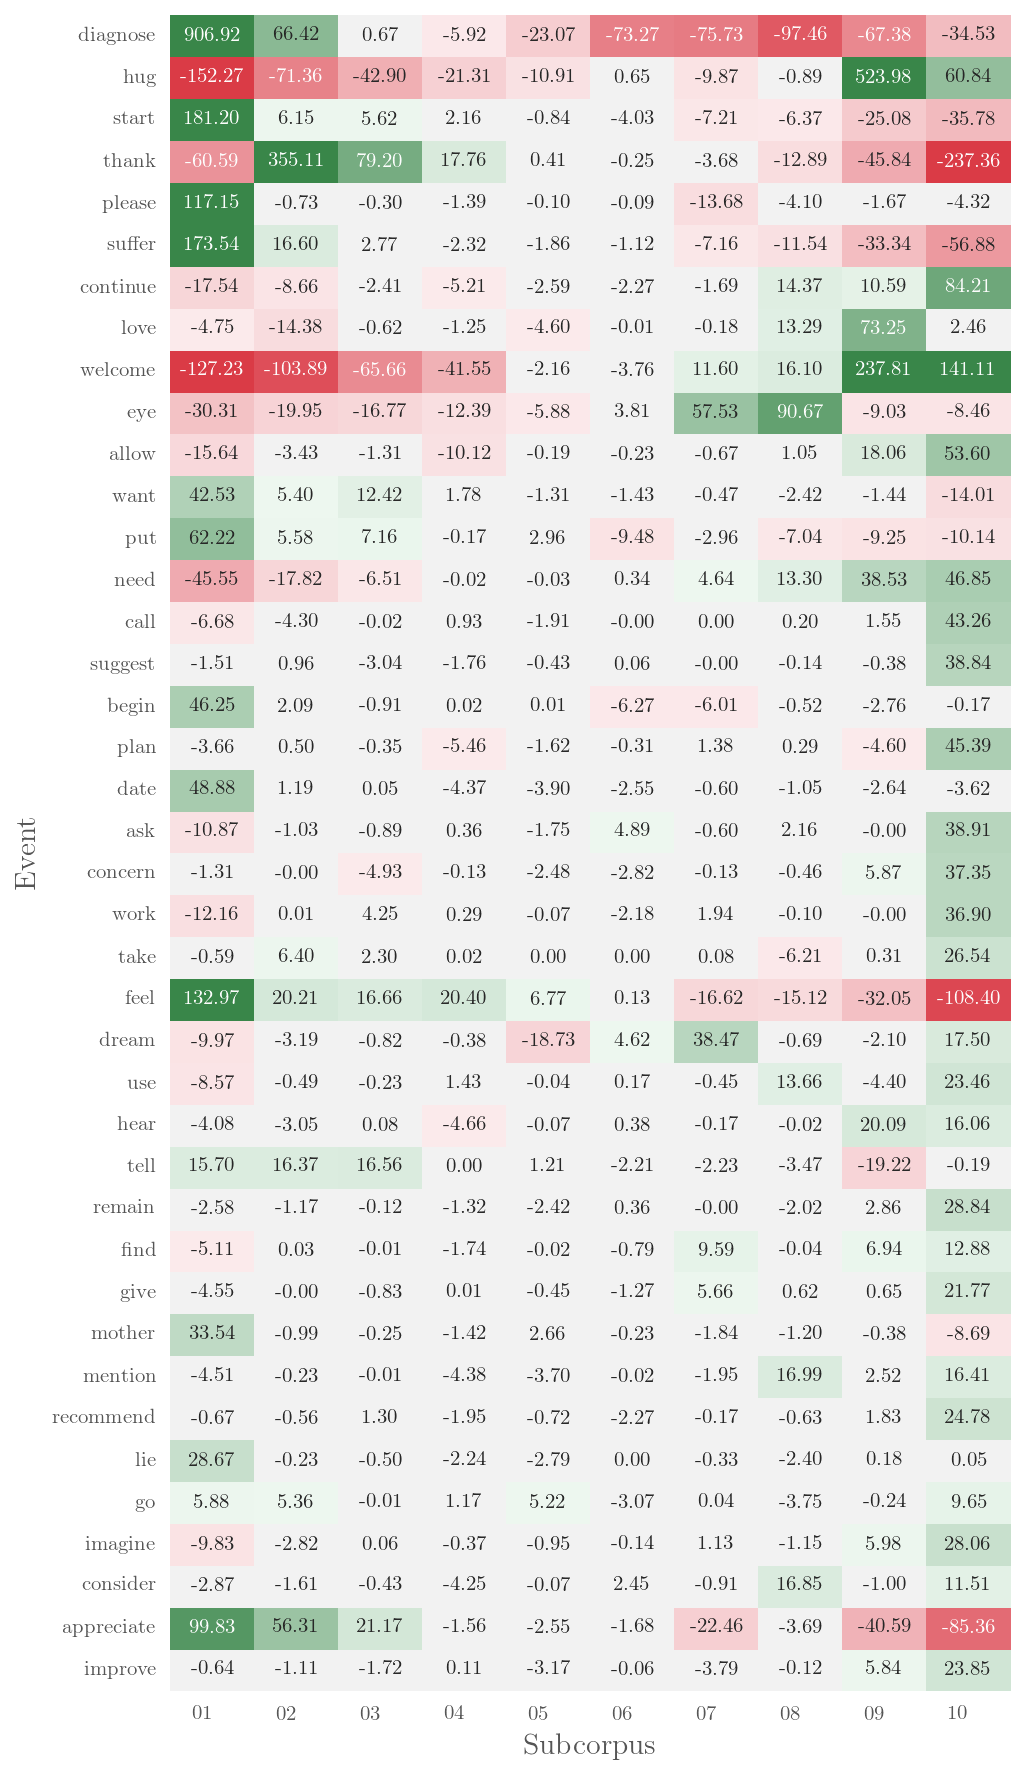
\includegraphics[width=0.80\textwidth]{images/event-heatmap.png}
    \hspace{1.6cm}
    \caption{Key and unkey Events in each subcorpus}
    \label{fig:event_heatmap}
 \end{figure}

Figure \ref{fig:event_heatmap} shows which Events are key in each subcorpus according to a log-likelihood comparison of the Forum contents as a whole. By far the most key process in any subcorpus is \emph{diagnose} in Subcorpus 01, as diagnosis is both the catalyst for visits to the site, and the main entry condition for participatory information and support exchange. Similarly, \emph{thank} is key in second post because users thank others for replies to their first. Other key Events in first post reveal different kinds of motivations for joining the community, including being \emph{told} that they may have bipolar, \emph{dates} with bipolar people, and \emph{beginning\slash starting} new medication regimens or manic\slash depressive cycles.

As with the analysis of participants, where veteran members orient toward more positive lexis, positive processes related to social support also become more common in veteran post (\emph{hug, thank, love, welcome}). Another focal point is processes urging others to carry on (\emph{continue, remain, improve}), which also have positive connotations. This contrasts with the negative sentiments inherent in \emph{suffer} (as in, \emph{to suffer from bipolar}), which is key in first post (see below for a more thorough treatment of the ways in which bipolar is ascribed to the self and others across membership stages). Finally, it is notable that \emph{thank} and \emph{appreciate} are unkey in the final stage of membership; the increased social status in the community means that platitudes, for veterans, are no longer obligatory to the same extent.

\subsection{Construing diagnosis} \label{sect:diag}

%Concordancing allows a window into the figures involving \emph{diagnose} in early and late stages of membership.

% Goal of \emph{diagnose} processes in three stages of membership
% Circumstances in \emph{diagnose} processes in three stages of membership
\begin{figure}[htb]
    \centering
    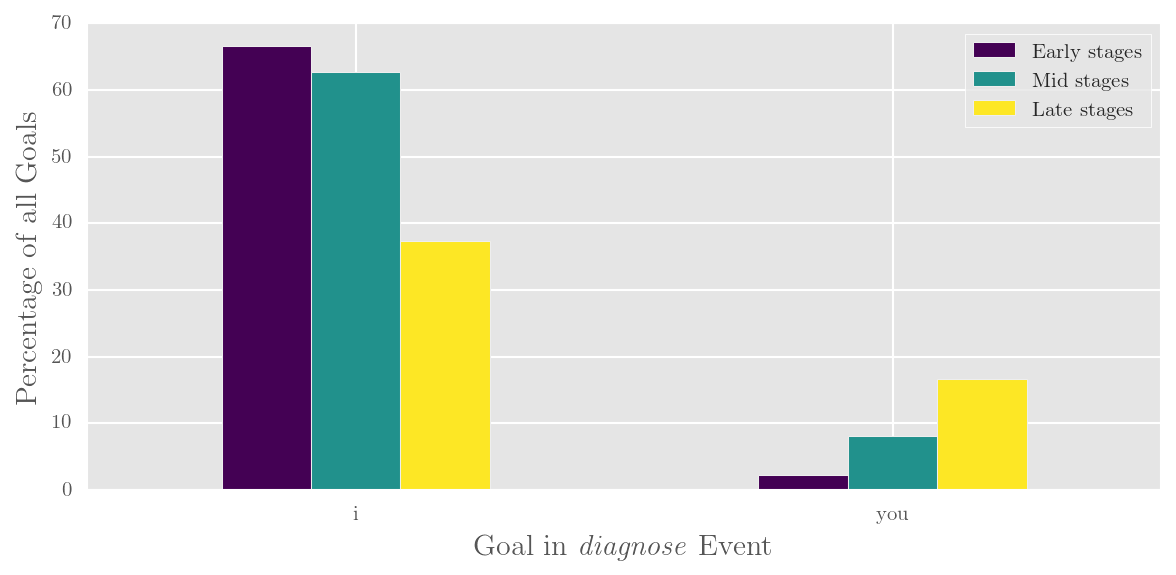
\includegraphics[width=0.8\textwidth]{images/goal-in-diag-ev.png}
    \caption[Goal of \emph{diagnose} processes]{Goal of \emph{diagnose} processes in three stages of membership}
    \label{fig:part_in_diag}
    \end{figure}

    \begin{figure}[htb]
    \centering
    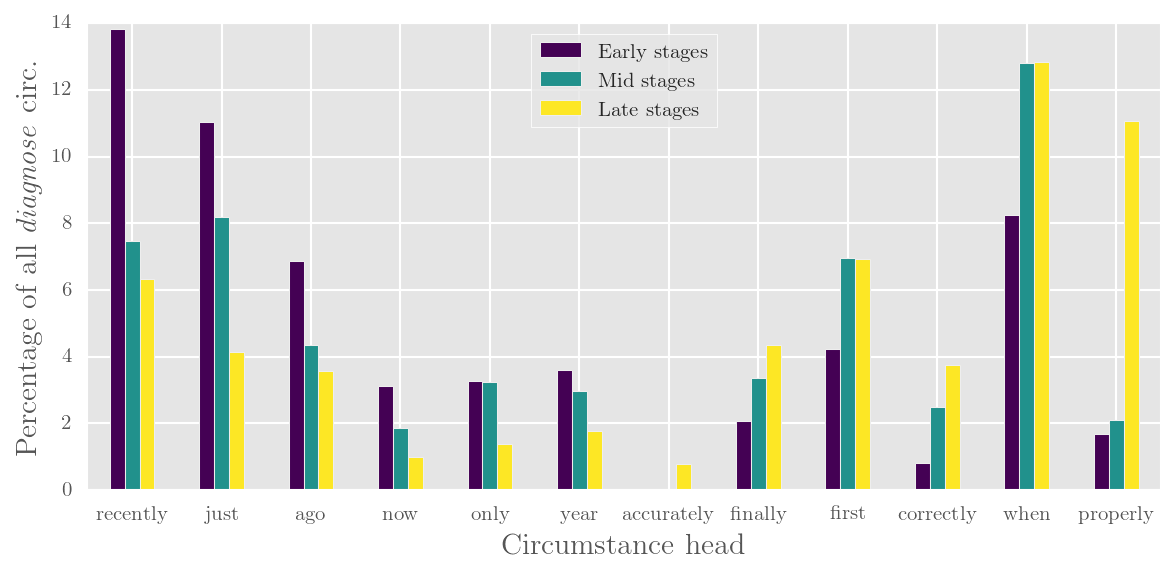
\includegraphics[width=0.8\textwidth]{images/diag-circ.png}
    \caption[Circumstances in \emph{diagnose} processes]{Circumstances in \emph{diagnose} processes in three stages of membership}
    \label{fig:circ_in_diag}
    \end{figure}

\emph{Diagnose} is a very prominent process in the Forum, and is by far the most key of key processes expressed in first posts. By contrasting early, middle and late stages of membership, clear differences emerge in how the process of diagnosis is configured over time (Figure \ref{fig:part_in_diag}). Veteran members, for example, are more likely to represent the health professional as the Actor in the \emph{diagnose} process. In terms of circumstances (Figure \ref{fig:circ_in_diag}), there is a shift in focus away from temporal meanings, with veteran members instead framing the \emph{diagnose} process with regard to its correctness, accuracy and legitimacy. New members often enter the community because of a recent or possible future diagnosis. Veterans, on the other hand, seek to ensure that the diagnosis is reliable. This has the dual purpose of ensuring the legitimacy of the new member's `entry ticket', and ensuring conformance with the biomedical model, where successful treatment is predicated on accurate diagnosis. Indeed, a number of users enter the community not because of a diagnosis from a health professional, but because they are attempting to ascertain whether their self-diagnosis, or their informal diagnosis of a friend or loved one, can stand up to the scrutiny of lay-experts. Veteran members, however, are reluctant to legitimise these kinds of strategies, due to their deviation from a normative conceptualisation of the `correct' consumer journey.

Notably, veteran members may deliberately undermine the biomedical model of diagnosis. While expressing conviction that diagnosis must be performed by a qualified health professional, they may simultaneously hint that the newcomer is \emph{probably} bipolar, or that non-bipolar diagnoses are in error. As was shown in the previous section, two separate replies to an undiagnosed newcomer relied upon the same lexicogrammatical means of hinting (\emph{It sounds like you might have bipolar to me}; \emph{if sounds very likely that you might have Bipolar disoder}), while nonetheless insisting on seeking diagnosis through mainstream channels (\emph{Find you a dr that can make a correct Diagnosis}; \emph{We aren't docs here and can't diagnose you}). This keeps the membership entry point open for those who have initially failed to meet the core criterion of a legitimate diagnosis, while pushing undiagnosed, suspected bipolar users toward actions that are in line with mainstream medical norms. %Help can be better provided once the condition is met.

\subsection{Diagnosis and grammatical metaphor}

Grammatical metaphor entails the use of one grammatical component to do the work that is congruently performed by another. Nominalisation is one of the most common examples \cite{simon-vandenbergen_grammatical_2003}. What is congruently an action, process or Event (e.g. to \emph{applaud}) may be reconstrued as a participant (\emph{applause}), allowing denser packaging of information. Turning the process into a participant also facilitates taxonomisation and classification: the lexical component of a nominal group may include Classifier, Epithet and Numerative, in addition to the Thing; in the verbal group, the only lexical component is the Event \cite{halliday_introduction_2004}. This kind of grammatical metaphor also opens up the reconstrued process to deixis.

Over the course of membership, the process of diagnosis undergoes a steady shift toward metaphorical realisation as a participant. In formal terms, it is more often nominalised. Figure \ref{fig:diag-gram-met} shows the strong relationship, but inexact, relationship between nominalisation and grammatical metaphor in the case of diagnosis: nominal and participant realisations become more frequent, while verbal and process realisations decrease. Charting experiential roles shows us that \emph{diagnose} is not limited to participant and process roles: commonly, it is a part of a circumstance (\emph{we received more help in terms of diagnosis and treatment}) or modifies a Thing (\emph{it is extremely common for those with undiagnosed bipolar disorder to self medicate}). The increasing extents to which \emph{diagnose} is nominalised, and to which \emph{diagnose} is represented as something other than a process, demonstrate an important discourse-semantic shift. By moving away from \emph{diagnose-as-process}, it becomes possible to represent diagnosis as a possession (\emph{it's great you have a final diagnosis and have started medication}), and therefore as something that can be acted upon or thought of in a particular way (\emph{i finally feel like i've accepted my diagnosis}). Another possibility opened up by nominalisation is the potential for modification through Epithets (\emph{this is a frightening diagnosis, particularly if you don't know anyone who has it}). Classification of \emph{diagnosis} through adjectival modification is also made possible (\emph{accurate}\slash \emph{correct} diagnosis), but, of course, as shown in Figure \ref{fig:circ_in_diag}, agnate meanings can be made through circumstantial modification of diagnose as a process (\emph{accurately\slash correctly diagnosed}). A final grammatical affordance is that diagnosis as a participant in a relational process can highlight its potential to be incorrect (\emph{my current diagnosis is schizo-affective disorder}; \emph{bp is becoming a catch-all diagnosis, frequently made by a well-meaning family doctor}). In this way, grammatical metaphor not only contributes to an increasingly scientised register, but also expands veteran members' ability to explain medical processes and their relationship to other members \cite{heyvaert_nominalization_2003}.

Calculating the relative frequencies of common modifiers of diagnose as verb (\emph{diagnose}, \emph{diagnosed}, \emph{diagnosing}) and diagnose as noun (i.e. diagnosis\slash diagnoses) clearly shows a preference for temporal modification of verbs and veracious modification of the nominal form (Table \ref{relfreq-diagnose-mods}).

%More generally, veterans may wish to invoke a scientised register, which 

% Grammatical metaphor in \emph{diagnosis}, via word classes and experiential roles
\begin{figure}[htb]
    \minipage{0.48\textwidth}\centering
    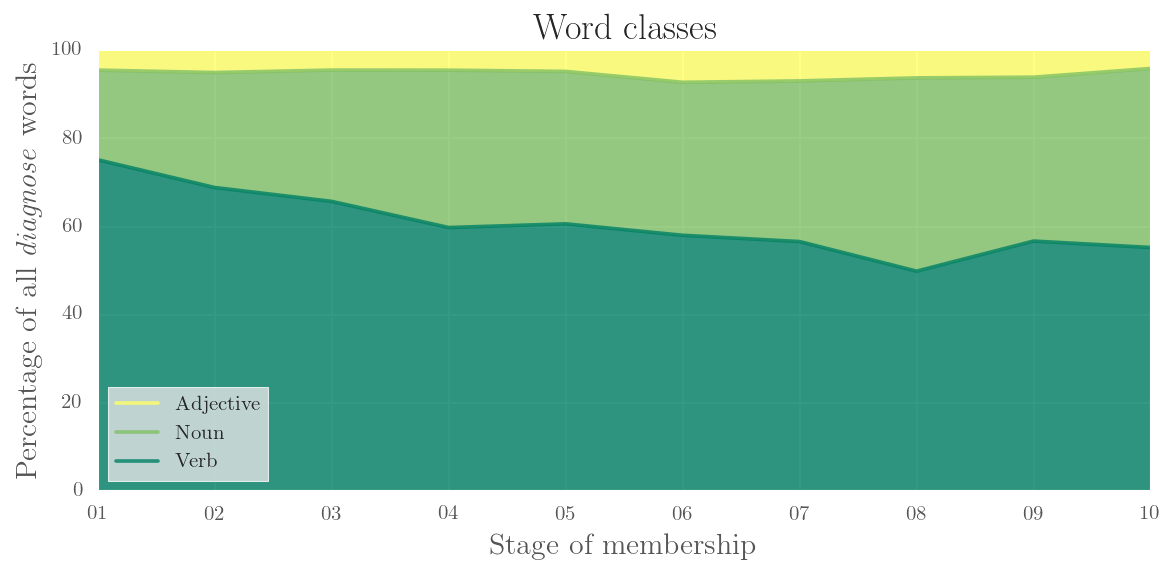
\includegraphics[width=1.00\textwidth]{images/wc-diag.png}
    \endminipage\hfill
    \minipage{0.48\textwidth}\centering
    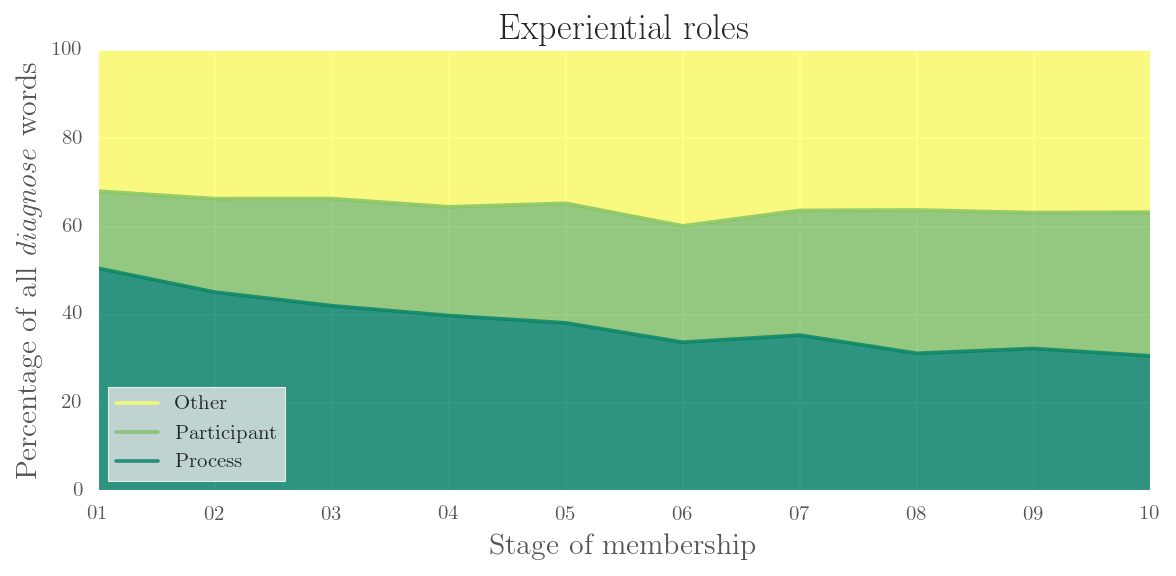
\includegraphics[width=1.00\textwidth]{images/exp-diag.png}
    \endminipage\hfill
    \caption[Grammatical metaphor in \emph{diagnosis}]{Grammatical metaphor in \emph{diagnosis}, via word classes and experiential roles}
    \label{fig:diag-gram-met}
    \end{figure}

\begin{table}[htb]
\begin{tabular}{lrlr}

\toprule
\emph{Diagnose}  & Rel freq.        & \emph{Diagnosis} & Rel. freq. \\
\midrule
not               &  11.80 & bipolar    &  11.13 \\
ago               &  11.10 & proper     &   8.82 \\
just              &   7.60 & correct    &   7.49 \\
recently          &   6.68 & dual       &   5.07 \\
when              &   4.16 & right      &   4.41 \\
now               &   3.54 & new        &   3.96 \\
only              &   3.11 & official   &   2.75 \\
properly          &   2.75 & different  &   2.64 \\
also              &   2.27 & wrong      &   2.20 \\
finally           &   2.12 & other      &   2.20 \\
so                &   2.09 & same       &   1.87 \\
never             &   2.09 & initial    &   1.65 \\
then              &   1.93 & possible   &   1.54 \\
correctly         &   1.50 & true       &   1.54 \\
well              &   1.47 & recent     &   1.43 \\
\bottomrule
\end{tabular}
\caption{Most common modifiers of \emph{diagnose} and \emph{diagnosis}}
\label{relfreq-diagnose-mods}
\end{table}

%todo: analysis of ajectives in diagnosis
Furthermore, they frame diagnosis as possibilistic: diagnoses can be \emph{suspected} or \emph{unofficial}. Such a framing is at odds with the normative biomedical model, however: informal kinds of diagnosis cannot be acted upon with appropriate treatment regimens. Veteran members therefore stress correct diagnosis in order to realign new members' construal of diagnosis with the ideology of the board. Though the focus of the community is on offering information and support for people with bipolar, those without official diagnoses ultimately cannot be helped \cite{vayreda_social_2009}. Ideologically, validation of community membership is withheld until new members have aligned with a normative biomedical trajectory that foremost involves diagnosis by professionals operating within a formal healthcare institution.


\section{Discussion}

\emph{Diagnose} as an Event was found to be a very key process in first contributions, leading to more delicate analysis of its behaviour in the corpus. This analysis turned up an increasing rate of grammatical metaphor (in the form of nominalisation, as \emph{diagnosis}), and shifts in attendant participants and circumstances. Each of these changes reflects a change in the discourse-semantics of the Event. First, the metaphorical realisation of the diagnosis Event as a participant opens it up to possession, deixis and more precise kinds of classification. At the beginning of membership, diagnosis is an Event that the speaker experiences, often without his\slash her volition, and often without an explicit Actor. The Event is situated in the past, represented as catalysing the new user's decision to sign up or contribute to the board. Diagnosis, as others have remarked, can function as a kind of entry ticket, or marker of legitimacy, for membership in mainstream OSGs \cite{stommel_use_2011}. Within the overarching ideology of the Forum, treatment \cite[including the talk therapy provided by Forum interaction itself---see][]{kaufman2016producing} is reserved for those who have an official mandate that warrants it \cite{vayreda_social_2009}. As such, it is no surprise that the \emph{diagnose} process is increasingly construed as a Thing that can be given, possessed and inspected. In the community, bipolar is understood to be treatable, but not curable---the amount of time between the diagnosis and the present is therefore more or less immaterial when inspecting the validity of the entry condition. Instead, what becomes important is the veracity of the diagnosis: \emph{suspected} and \emph{unofficial} diagnoses must become \emph{proper} and \emph{official} diagnoses, because it is correct diagnosis that steers the newcomer on the optimal path within the bipolar journey.

\section{Future directions}

This study has highlighted the utility of functional grammar and computational methods in interpreting online health discurse. At the same time, it demonstrates that many of the kinds of results that typically come from qualitative analysis can to some extent be automated, increasing reliability, reducing the potential for bias introduced either by researcher or sampling. Because the methods for data collection and analysis are automated and open-source, reproducing the analysis pipeline on other communities is trivial. This would facilitate multilingual studies, or studies of different health conditions. Alternatively, using the methodoligcal pipeline developed here, focus could switch from \emph{diagnosis} to another key event in health journeys (such as \emph{relapse}, in a forum for substance abuse, or \emph{remission}, in a cancer community).

Finally, a number of more novel computational methods could potentially be used. While the focus of this study was on lexicogrammatical analysis of parsed data, methods such as topic modelling and word vectors could provide novel insights into relationships between texts or word usages within large online collections of language. Given that these approaches typically do not involve annotation of text with theoretical models of language, they may well be an important step toward more complete automation of health language analysis. This broadens the explanatory power of functional and corpus linguistics, and moves closer toward research methods with valid implications for medical practice and policy.

\printbibliography[heading=bibintoc]

\end{document}